\section{Introduction}

Recently, coding agents~\cite{openai_codex,anthropic_claude_code} have shown remarkable capabilities in developing complex software systems, sparking growing interest in solving robotic manipulation tasks through programming~\cite{chen2026gap,xiao2026enpire,lu2026aspire,fu2026cap,berman2026claude,noematrix2026roborsi,liang2023code}. Consider how human engineers would develop a robot program to solve the task in Figure~\ref{fig:teaser} before the era of coding agents: given the \textit{(a) task specification} (pick up the cookie box), they would write a program that composes the available \textit{(b) manipulation primitives} (push the box to a fixture, flip it against the fixture, then grasp and lift it), and test the program in \textit{(c) interactive environments} to verify its correctness and iteratively debug it. This process mirrors the core strength of coding agents: not one-shot code generation, but the iterative cycle of generating, executing, verifying, and revising a program, commonly referred to as the agentic coding loop~\cite{ng2026three,huang2023agentcoder}.

For the agentic coding loop to work in robotic manipulation, it requires three ingredients: task specification, manipulation primitives, and interactive environments for verification. Existing robotic coding-agent systems typically assume these ingredients are provided through human-engineered primitives, explicit task objectives, and resettable environments with reward or success feedback. This raises a fundamental question: \textbf{how can a coding agent close the loop when these ingredients are not provided a priori?}

We explore \textit{demonstrations} as a programming interface for supplying the task- and motion-level information needed by the agentic coding loop. A demonstration directly shows a feasible way to accomplish a task and, together with a language description, conveys the intended outcome. Rather than merely reproducing the demonstrated trajectory, we aim to recover an executable and reusable manipulation program. Demonstrations, however, do not provide the interactive environment needed to verify and iteratively refine that program, posing an additional challenge for verification.

\begin{figure}[t]    
    \centering
    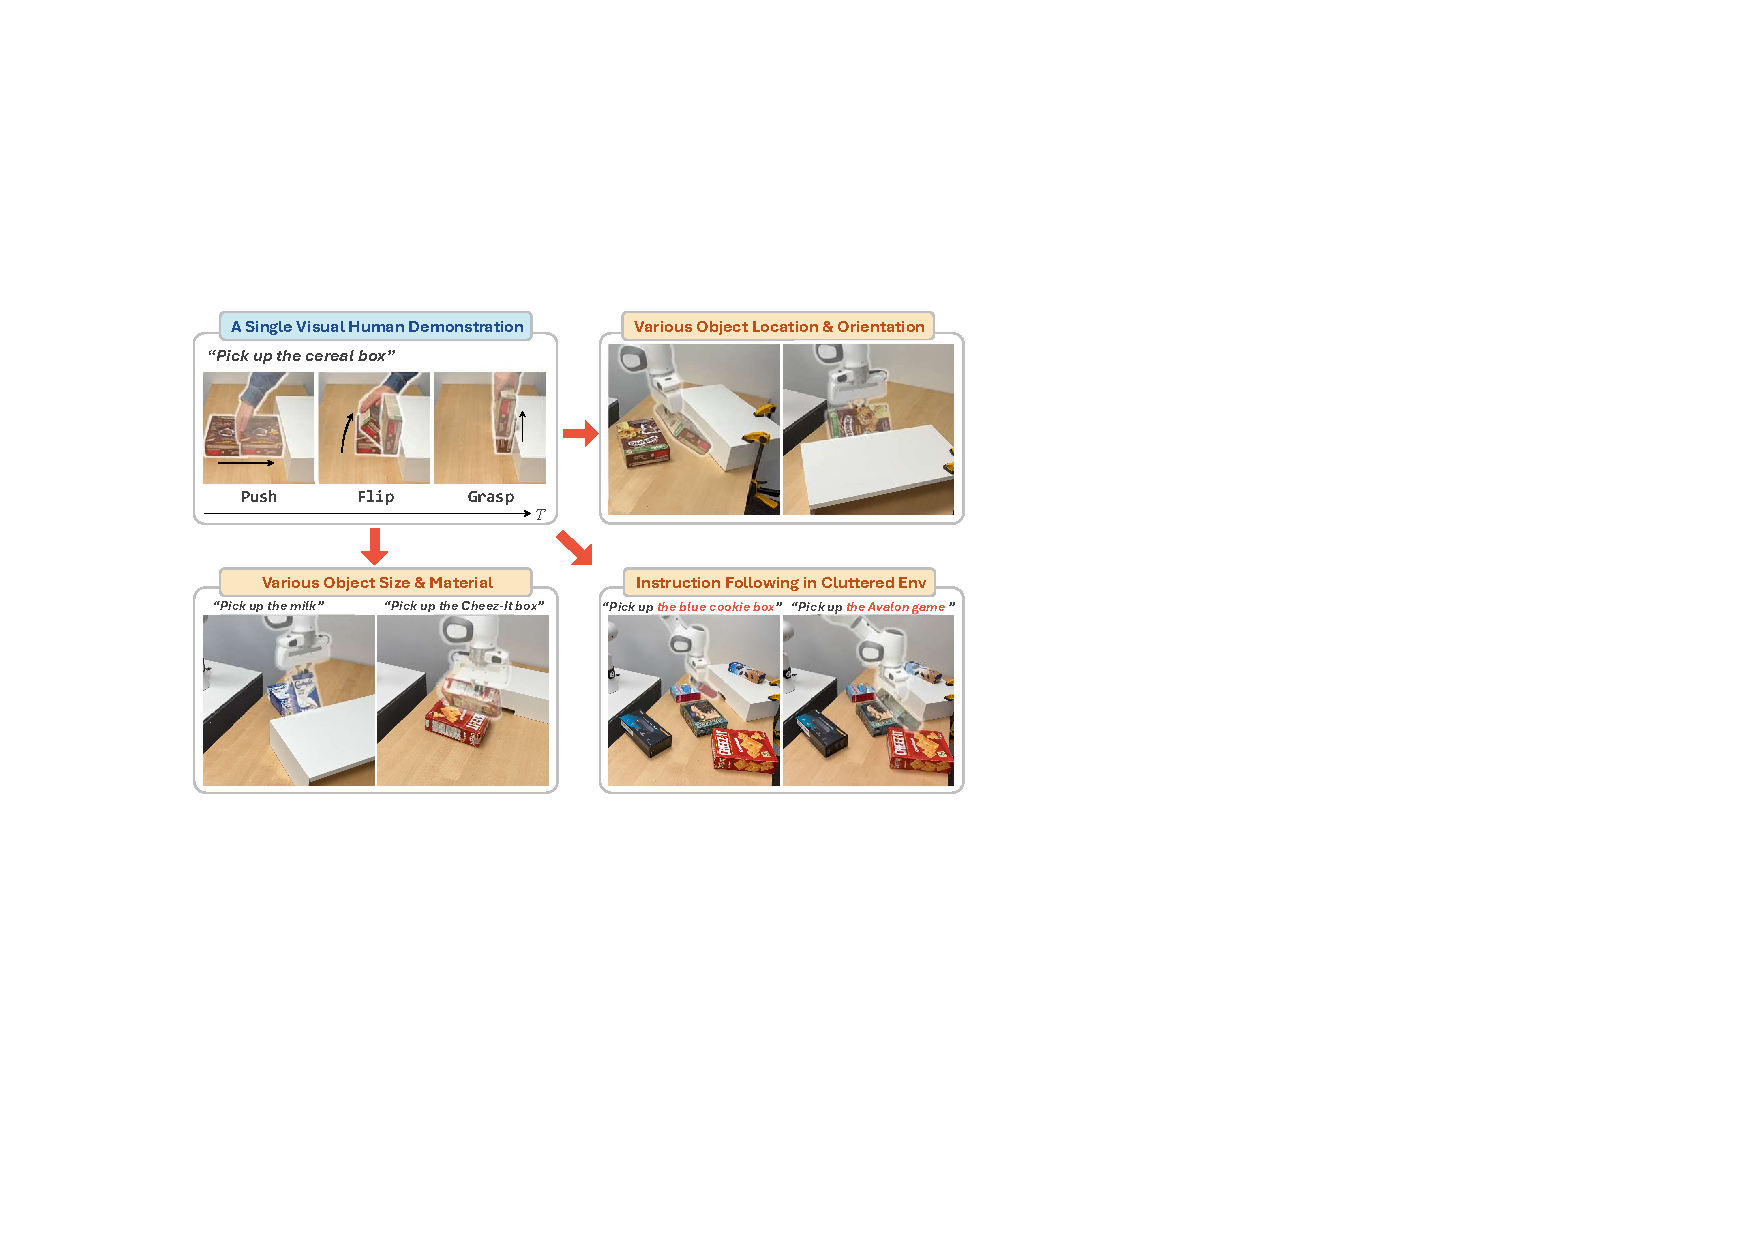
\includegraphics[width=\linewidth]{figures/teaser.pdf}
    \caption{teaser}
    \vspace{-0.3in}
    \label{fig:teaser}
\end{figure}

Motivated by this perspective, we introduce \textbf{R}obot \textbf{A}gentic \textbf{P}rogramm\textbf{i}ng from \textbf{D}emonstrations (\textbf{RAPID}), a framework for constructing and iteratively refining robot programs from a single human demonstration with a coding agent. RAPID infers the task specification, constructs the required manipulation primitives and strategy, and reconstructs the demonstrated scene in simulation for iterative program verification and refinement. To improve generalization, RAPID additionally generates scene variants for further verification. In this way, RAPID automatically establishes the three ingredients required to close the agentic coding loop for robotic manipulation.

In this work, we apply RAPID to \textit{nonprehensile manipulation}, where the need for such a framework is especially acute. Many prehensile tasks can be composed from a compact and well-established set of reusable primitives~\cite{garrett2021integrated}, including \textit{pick}, \textit{move in free space}, and \textit{place}. Nonprehensile manipulation, by contrast, spans diverse and geometry-dependent contact interactions, including pushing~\cite{mason2001mechanics}, pivoting~\cite{holladay2015general}, toppling~\cite{cheng2021contact}, flipping~\cite{odhner2013open}, and sliding~\cite{cheng2022contact}. Capturing this diversity with a fixed primitive library is difficult, making manual primitive design a significant engineering burden. This makes nonprehensile manipulation a natural testbed for asking whether a coding agent can construct reusable manipulation primitives from a single demonstration rather than rely on human engineering.

A central challenge is \textit{generalization} beyond a single demonstrated scene. Programs that directly encode poses, distances, or waypoints may reproduce the demonstrated behavior but can fail when the scene changes. RAPID instead captures the behavior in terms of object-centric relations and task-relevant effects. Specifically, RAPID represents primitives as relational trajectory-optimization programs that realize object-level motion effects, such as pushing an object by a displacement or flipping it by an angle, while resolving scene-dependent geometry at execution time. At the task level, primitives are connected into a strategy through relational constraints that determine how the outcome of one phase specifies the next. For example, rather than replaying a fixed pushing distance, the program can compute how far an object should be pushed from its current pose to establish contact with a fixture. By expressing primitives and their composition relationally, RAPID preserves the invariant structure of the demonstrated strategy while adapting to changes in object pose, size, geometry, and physical properties.

The remaining challenge is \textit{verification}: the coding agent needs an interactive environment in which candidate programs can be executed, evaluated, and revised. RAPID reconstructs such an environment in simulation from the demonstration and augments it with scene variants that perturb object geometry, pose, appearance, and physical properties. Agent-generated filters retain only task-consistent and physically feasible variants. The coding agent then executes and iteratively revises the program across this verification set. This simulation-based verification closes the agentic loop while reducing overfitting to the demonstrated scene.

We evaluate RAPID on 8 contact-rich nonprehensile manipulation tasks, focusing on whether a program constructed from one demonstrated instance can generalize to substantial changes in object pose, geometry, physical properties, and scene configuration. We additionally evaluate the frozen programs on physical robots and conduct ablations to assess the contributions of the relational program representation, scene variation, and iterative verification.

Our contributions are threefold:

\begin{itemize}

\item We introduce RAPID, a framework that closes the agentic coding loop for robotic manipulation by automatically constructing \textit{(a) task specifications}, \textit{(b) manipulation primitives}, and \textit{(c) interactive verification environments}, all from a single human demonstration.

\item We introduce \textit{relational manipulation programs}, which represent manipulation primitives as parameterized trajectory-optimization programs and compose them through relational constraints, enabling reusable strategies that adapt across scenes.

\item We demonstrate that RAPID can construct reusable programs from a single human demonstration across diverse contact-rich nonprehensile manipulation tasks, generalize to substantial scene variations, and be deployed in the real world.

\end{itemize}
